\section{OpenVPN}
Dopo aver scartato SoftEther, si è iniziato a testate OpenVPN. Prima di passare a
descrivere la configurazione
utilizzata, è utile fare un breve riepilogo ed approfondamento su come OpenVPN
funzioni. Già in questo capitolo si discute della sicurezza di OpenVPN; tuttavia
si rimanda al capitolo \ref{chap:security} per un'analisi approfondita.

\subsection{Introduzione}
OpenVPN è una tecnologia VPN diffusa ed accettata, in grado di realizzare
diverse topologie, incluse l'accesso remoto ed LAN-to-LAN, può incapsulare il
livello 2 o al livello 3 dello stack ISO/OSI, e come protocollo di trasporto
può utilizzare TCP oppure UDP. OpenVPN è estremamente configurabile, e per questo
motivo è molto flessibile, ciò è uno dei suo maggiori punti di forza.\\
OpenVPN utilizza due canali tra i due peer, multiplexati su una singola connessione
TCP/UDP. Essi sono:
\begin{itemize}
	\item \texttt{Control Channel} una connessione cifrata con TLS utilizzata tra i
	      partecipanti per scambiarsi informazione di \textit{servizio}, come configurazioni
	      inviate da server a client e negoziazione delle chiavi.
	\item \texttt{Data Channel} la connessione su cui sono effettivamente scambiati
	      i dati della VPN, protetta con un protocollo simile a TLS.
\end{itemize}
Il \texttt{Control Channel} garantisce tutte le proprietà di sicurezza di TLS,
tra cui ovviamente autenticazione, confidenzialità ed integrità
dei dati scambiati.
utilizzando un algoritmo di cifratura a chiave simmetrica combinato
con un MAC.

Poiché i due canali sono multiplexati sulla stessa connessione, OpenVPN aggiunge
il proprio header dopo l'header del protocollo di livello 4. Il payload del
protocollo OpenVPN contiene quindi i dati del \texttt{Control}
e del \texttt{Data Channel} come mostrato in figura \ref{fig:openvpn-tunnelling}.

\begin{figure}[h!]
	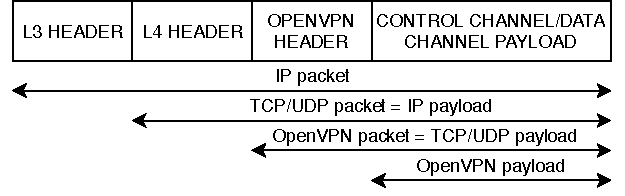
\includegraphics[scale=0.85]{img/openvpn_tunnelling}
	\caption{Struttura di un pacchetto OpenVPN}
	\label{fig:openvpn-tunnelling}
\end{figure}

Una volta che il normale TLS handshake viene portato a termine ed il \texttt{Control Channel}
è in funzione, OpenVPN genera delle chiavi simmetriche da utilizzare per proteggere
il \texttt{Data Channel}. Contrariamente al TLS handshake in cui si utilizza Diffie-Hellman
come \textit{base} per derivare le chiavi di sessioni, nel \texttt{Data Channel} le
chiavi sono una semplice \textit{composizione} di byte pseudo casuali generati
dalla libreria TLS usata da OpenVPN. Queste chiavi
vengono scambiate nel \texttt{Control Channel}, ed entrambi i partecipanti contribuiscono
nel materiale pseudo casuale.\\
A questo punto si può dire che l'intero handshake sia stato completato, e che le parti
dispongano delle seguenti chiavi:
\begin{itemize}
	\item $A_{Ctrl\_Chan} \rightarrow B_{Ctrl\_Chan}$
	\item $B_{Ctrl\_Chan} \rightarrow A_{Ctrl\_Chan}$
	\item $A_{Data\_Chan} \rightarrow B_{Data\_Chan}$
	\item $B_{Data\_Chan} \rightarrow A_{Data\_Chan}$
\end{itemize}
Ci sono casi in cui le chiavi non sono quattro in tutto ma bensì otto, ciò dipende
dal fatto che si utilizzi una ciphersuite che fornisca in un'unica costruzione \textit{Authenticated
	Encryption (with Associated Data)} (come \texttt{AES-GCM} o \texttt{ChaCha20-Poly1305})
	oppure una in cui
occorra combinare un cifrario ed un algoritmo di MAC, come \texttt{AES-CBC-HMAC-SHA256}.
Entrambi i canali di OpenVPN garantiscono \textit{Authenticated Encryption}.
Tutte le operazioni crittografiche sono effettuate mediante librerie esterne,
attualmente OpenVPN supporta le seguenti tre:
\begin{itemize}
	\item \texttt{OpenSSL}\footnote{\url{https://www.openssl.org/}}
	\item \texttt{LibreSSL} (fork di \texttt{OpenSSL}, supportata non ufficialmente)\footnote{\url{https://www.libressl.org/}}
	\item \texttt{mbedTLS}\footnote{\url{https://tls.mbed.org/}}
\end{itemize}

E' possibile autenticare i partecipanti alla VPN mediante
certificati X509 oppure medianti chiavi simmetriche precondivise. Nel caso di MoonCloud
si è scelta la prima opzione poiché garantisce \textit{Perfect Forward Secrecy}.


OpenVPN è disponibile in due versioni: una gratuita ed una a pagamento denominata
``\textit{Access Server}'', la quale offre una interfaccia web per configurare il server.
E' stato scelto di utilizzare la versione gratuita (``\textit{Community Edition}''),
e come tale per poter essere configurata si utilizzano uno o più file di configurazione.\\
A partire dalla versione 2.0, OpenVPN è una VPN \textit{client-server}, nel senso che
vi è un host che svolge il ruolo di server ed accetta più connessioni provenienti
dai client. Una volta che tale connessione è stata stabilita, client e server
possono essere considerati dei \textit{peer} poiché entrambi possono mandare pacchetti
all'altro, senza necessità che un client richieda qualcosa ed il server vi risponda
(come in un tradizionale protocollo client-server). Per questo si utilizzerà
il termine ``peer'' quando non sarà necessario distinguere chi sia il client e chi
il server.



OpenVPN ricalca esattamente il funzionamento ``tipico'' di una VPN, in cui server e client
sono connessi mediante socket su un protocollo di trasporto, ed i pacchetti scambiati
lungo tale socket sono cifrati.
Su questo collegamento vi sono quei pacchetti provenienti dalla rete a cui uno di essi
appartiene e destinati all'altra. Ciascun partecipante crea quindi una scheda di rete
virtuale a cui invia i pacchetti destinati ad host delle propria rete, e riceve
pacchetti provenienti da essi e destinati alla rete del client.\\
Si esamina ora il flusso che compie un pacchetto generato da un certo host nella rete
del server e destinato ad un host nella rete del client.
\begin{enumerate}
	\item Il pacchetto viene ricevuto dalla scheda di rete fisica del server e passa
	      al kernel del sistema operativo
	\item il sistema operativo provvede ad inoltrare il pacchetto alla scheda di rete
	      virtuale del VPN server
	\item il processo OpenVPN riceve il pacchetto, esso è composto dall'header IP come
	      protocollo di più basso livello
	\item il processo verifica a quale client inoltrare il pacchetto sulla base delle rotte
	      interne configurate
	\item il pacchetto viene inviato cifrato al client designato lungo il socket. Nello
	      specifico, \textit{il vecchio pacchetto viene incapsulato in un nuovo pacchetto,
	      	ed il pacchetto incapsulato è cifrato, diventando il payload del pacchetto
	      	più esterno}\footnote{Ciò che si è descritto, ovvero incapsulare un pacchetto di rete
	      	in un altro pacchetto facendolo diventare il payload di quest'ultimo, viene detto
	      	\textit{tunneling}.}.
	\item il pacchetto, dopo aver attraversato Internet, viene ricevuto dalla scheda di rete
	      fisica del client
	\item il sistema operativo lo inoltra quindi al socket del client
	\item il client decifra il pacchetto e lo scrive sulla sua scheda di rete virtuale
	\item il sistema operativo ``riceve'' il pacchetto e vi applica il routing, quindi
	      lo inoltra alla scheda di rete fisica dell'host
	\item il pacchetto viene infine ricevuto dal destinatario
\end{enumerate}
Il pacchetto ricevuto al punto \textit{1} è esattamente identico a quello del
punto \textit{10}.
Tutto ciò presuppone che siano configurate le seguenti rotte:
\begin{itemize}
	\item nella rete del server:
	      \begin{itemize}
	      	\item \textit{destinazione: rete-client, via: VPN server}; questa configurazione
	      	      può essere fatta su ogni host della rete oppure sul default gateway
	      \end{itemize}
	\item nella rete del client analogamente:
	      \begin{itemize}
	      	\item \textit{destinazone: rete-server, via: VPN client}
	      \end{itemize}
\end{itemize}
il VPN server deve essere inoltre configurato per sapere quali client sono responsabili
per quali reti (le cosìdette ``\textit{rotte interne}'').


\subsection{Configurazione base}
In questa sottosezione si propongono due esempi di una configurazione ``tipica''
e minimale per OpenVPN per realizzare una topologia LAN-to-LAN. Si riporta il
contenuto dei file di configurazione di client e server, ciascuna entry sarà quindi discussa in dettaglio.
Si supponga che la sottorete del server abbia il seguente indirizzo: \texttt{192.169.100.0/24},
mentre quella del client sia: \texttt{192.168.1.0/24}. Il server è raggiungibile
tramite l'IP pubblico \texttt{11.9.250.34}.

\subsubsection{Configurazione del server}
Ecco come si potrebbe presentare
il file di configurazione del server.
\begin{minted}{squidconf}
mode server
tls-server
	
# il protocollo L4
proto tcp
	
# il tipo di scheda di rete virtuale
# ed il suo nome
dev-type tun
dev server
	
persist-tun
persist-key

script-security 2
	
# privileges downgrading
group nogroup
user nobody
	
# porta di ascolto
port 443
	
# VPN subnet
server 10.7.0.0 255.255.255.0
	
# topologia
topology subnet
client-to-client
	
# configurazioni TLS
remote-cert-eku "TLS Web Client Authentication"
tls-version-min 1.2
tls-cipher TLS-ECDHE-ECDSA-WITH-AES-256-GCM-SHA384
cipher AES-256-GCM
	
# certificato CA
ca /etc/openvpn/certs/ca.crt
	
# key/cert di questo server
key /etc/openvpn/server/server.key
cert /etc/openvpn/server/server.crt
	
# ECDH anziché DH
dh none
	
# nuove chiavi Data Channel ogni 20 minuti
reneg-sec 1200
	
# configurazioni log
log /var/log/openvpn/openvpn-server.log
verb 4
status /var/log/openvpn/openvpn-status.log
	
# configurazioni keepalive
keepalive 10 60
	
# informazioni di routing
push "route 192.168.100.0 255.255.255.0"
route 192.168.1.0 255.255.255
	
# spiegato poi
client-config-dir /etc/openvpn/server/ccd
\end{minted}
Si supponga infine che il \texttt{CommonName} nel certificato del client sia
``\texttt{client1}'', e che esista un file al percorso
``\path{/etc/openvpn/server/ccd/client1}''. Tale file avrà questo contenuto:
\begin{minted}{squidconf}
	iroute 192.168.1.0 255.255.255.0
\end{minted}
Linea per linea si descrive il contenuto del file:
\begin{description}
	\item[\texttt{mode server}]Indica che OpenVPN opera in modalità server.
	\item[\texttt{tls-server}]Questa direttiva specifica quale sia il ruolo nel TLS
	handshake.
	\item[\texttt{proto tcp}]Indica qual'è il protocollo di trasporto utilizzato,
	in questo caso è TCP.
	\item[\texttt{dev-type tun}]Quale tipo di scheda di rete virtuale utilizzare:
	\texttt{TUN} è un modulo del kernel utilizzato per creare interfacce di rete virtuali
	al livello 3.
	\item[\texttt{dev server}]La direttiva ``\texttt{dev}'' indica che nome dare
	alla scheda di rete virtuale, in questo caso la si chiama ``\texttt{server}''.
	\item[\texttt{persist-tun}]Specifica di non chiudere e riaprire la scheda di rete
	virtuale tra i vari restart.
	\item[\texttt{persist-key}]Similmente alla precedente, dice di non rileggere la chiave privata quando una
	sessione VPN finisce, o quando si ricevono particolari segnali dal sistema operativo.
	\item[\texttt{script-security 2}]Specifica quale tipo di programmi esterni è consentito
	chiamare, in questo caso si consentono script definiti dall'utente.
	\item[\texttt{group nogroup}, \texttt{user-nobody}]Questa direttiva fa
	sì che una volta partito, OpenVPN
	non abbia più privilegi amministrativi.
	\item[\texttt{port 443}]Specifica su quale porta il server si deve mettere in ascolto per
	ricevere connessioni dai client.
	\item[\texttt{server 10.7.0.0 255.255.255.0}]Questa direttiva indica che la sottorete
	assegnata al collegamento VPN è quella indicata.
	\item[\texttt{topology subnet}]Indica di allocare un indirizzo IP alla scheda
	di rete virtuale, esso appartiene al pool di IP presente nella direttiva \texttt{server}.
	Il server avrà come IP il primo IP disponbile nella sottorete (quindi \texttt{10.7.0.1}).
	\item[\texttt{client-to-client}]Si usa questa opzione per realizzare una connettività
	completa tra le diverse reti client: se viene inserita nel file di configurazione essa
	specifica che il server può fare il routing dei pacchetti \textit{tra} i client, e non
	solo tra i client ed il server stesso.
	\item[\texttt{remote-cert-eku "TLS Web Client Authentication"}]Direttiva che specifica
	di che ``tipo'' deve essere il certificato dei client che si connettono, è un'opzione
	non obbligatoria ma che migliora la sicurezza.
	\item[\texttt{tls-version-min 1.2}]Come si può immaginare, indica quale versione minima
	del protocollo TLS si deve usare. TLS 1.3 è già diventato standard, ma attualmente
	non è ancora supportato \cite{RFC8446}.
	\item[\texttt{tls-cipher TLS-ECDHE-ECDSA-WITH-AES-256-GCM-SHA384}]Questa direttiva
	indica quali ciphersuite di TLS utilizzare nel \texttt{Control Channel}\footnote{E' bene
		verificare quale versione di OpenVPN sia in uso e con quale libreria TLS sia
		stata compilata per una lista completa degli algoritmi supportati.}.
	\item[\texttt{cipher AES-256-GCM}]La direttiva \texttt{cipher} specifica
	quale algoritmo, ed in quale modalità, usare per il \texttt{Data Channel}.
	\item[\texttt{ca /etc/openvpn/certs/ca.crt}]Specifica il percorso a cui si trova
	il certificato della CA usato per creare i certificati dei client. E' indispensabile
	ai fini della validazione degli stessi.
	\item[\texttt{key /etc/openvpn/server/server.key}, \texttt{cert /etc/openvpn/server/server.crt}]
	Indica il percorso a cui si trovano,
	rispettivamente, la chiave privata del server ed il suo certificato.
	\item[\texttt{dh none}]Normalmente OpenVPN negozia le chiavi utilizzando il \textit{normale}
	Diffie-Hellman (aritmetica modulare, utilizzando numero primo), e richiede che i parametri
	per tale \textit{key agreement} siano generati a priori. Se si vuole utilizzare
	Diffie-Hellman su curva ellittica (\textit{ECHD}) occorre specificare ``\texttt{none}''
	come parametro a ``\texttt{dh}''.
	\item[\texttt{reneg-sec 12000}]Le chiavi del \texttt{Data Channel} sono di default rinegoziate
	ogni ora, volendo essere particolarmente conservativi, si può configurare
	la rinegoziazione ogni 20 minuti (o un qualsiasi altro valore), come fatto in
	questo caso. E' sufficiente specificare questa configurazione su un partecipante
	alla VPN, l'host con la soglia più bassa scatenerà una rinegoziazione.
	\item[\texttt{log /var/log/openvpn/openvpn-server.log}]Questa direttiva specifica
	il percorso del file di log.
	\item[\texttt{verb 4}]Specifica il livello di verbosità del log, un livello di
	4 o 5 è considerato adeguato in produzione, livelli più alti (disponibile fino al 9)
	sono utilizzati per il debugging.
	\item[\texttt{status /var/log/openvpn/openvpn-status.log}]Questa direttiva indica
	quale è il file di \textit{status} in cui OpenVPN scrive informazioni relative
	alle connessioni con i client.
	\item[\texttt{keepalive 10 60}]La direttiva ``\texttt{keepalive}'' indica ogni
	quanto OpenVPN deve mandare dei \textit{keepalive} al peer a cui è connesso.
	Il primo parametro indica ogni quanto mandare dei keepalive (in secondi), mentre
	il secondo indica dopo quanti secondi considerare la connessione caduta se non riceve
	niente dal client a cui è connesso. E' sufficiente specificare questa opzione
	nel server, esso provvederà a trasmetterla al client.
	\item[\texttt{push "route 192.168.100.0 255.255.255.0"}]Questa direttiva viene
	usata lato server per inviare delle configurazioni ai client. In questo caso si indica
	ai client di aggiungere nella routing table del sistema operativo una rotta che
	apparirà così: \texttt{rete 192.168.100.0/24 via <virtual NIC's IP>}. Essendo
	\texttt{192.168.100.0/24} la rete in cui si trova il server, l'effetto di questa
	rotta è che ogni volta che l'OS deve decidere dove inoltrare un
	pacchetto destinato a tale rete, lo invii alla scheda di rete virtuale
	del client. In questo modo il client VPN lo riceve da essa e lo invia al server
	lungo il socket.
	\item[\texttt{route 192.168.1.0 255.255.255}]Indica di aggiungere una rotta
	così composta nella routing table dell'OS del server: \texttt{rete 192.168.1.0/24
		via <virtual NIC's IP>}. Poiché \texttt{192.168.1.0/24} è la rete del client, l'effetto
	dell'aggiunta di questa rotta è l'analogo di quello visto al punto precedente, solo che
	viene applicato localmenete.
	\item[\texttt{client-config-dir /etc/openvpn/server/ccd}]Specifica in quale
	directory si trovano i file contenenti configurazioni specifiche per ciascun client.
	Tale directory conterrà una serie di file i quali dovranno chiamarsi semplicemente
	come il \texttt{CommonName} dei certificati dei client. La principale e più
	importante direttiva nei suddetti file è descritta nel punto successivo.
	\item[\texttt{iroute 192.168.1.0 255.255.255.0}]E' molto importante comprendere
	il significato di questa direttiva e capire che essa si trova dentro un file
	contente configurazioni specifiche per un certo client. ``\texttt{iroute}'' seguito
	da un indirizzo di rete, indica che \textit{il client a cui il file di configurazione
		si riferisce è responsabile per la rete \texttt{192.168.1.0/24}}. Mediante le
	direttive \texttt{iroute}, OpenVPN costruisce una routing table interna,
	e tramite essa si
	decide a quale client inviare un certo pacchetto. Bisogna infine tener presente
	che occorre anche la direttiva \texttt{route \ldots}, poiché essa agggiunge delle
	rotte alla routing table del sistema operativo, mentre \texttt{iroute} solo
	alla routing table di OpenVPN.
\end{description}

\subsubsection{Hook}
Oltre alle configurazioni \textit{tipiche} appena mostrate, ve ne sono molte altre. In effetti,
uno dei punti di forza di OpenVPN è proprio l'elevatissima configurabilità.
Tra le altre cose consente di definire una serie di \textit{hook},
cioè azioni da eseguire (lanciare programmi esterni) quando alcuni eventi si verificano.
Esistono degli hook ben precisi, alcuni dei quali sono effettivamente utilizzati
nella configurazione di MoonCloud. Per ciascun hook si specifica nel file di configurazione
quale azione compiere, cioè quale programma deve essere eseguito.

I programmi lanciati, tipicamente file di testo in un linguaggio di scripting, devono 
terminare con un valore di uscita secondo
la classica semantica per cui \texttt{0} indica \textit{successo}, un qualsiasi
altro valore \textit{fallimento}. Molti di questi hook sono disponibili solo in modalità
server. Alcuni di essi possono essere usati per validare il collegamento con
un client: nel momento in cui OpenVPN riceve una connessione può invocare uno (o più)
script, ed un valore di ritorno \texttt{0} indica di continuare il collegamento, e viceversa.

Ogni script invocato ha a disposizione un certo numero di variabili d'ambiente settate
da OpenVPN.

% Sulla base
% di esso OpenVPN decide se proseguire nella connessione con un remote oppure terminarla.
% Alcuni hook sono disponibili solo in modalità server, in tal caso
% l'idea sarebbe quella di decidere se consentire ad un client di portare avanti
% la connessione al server oppure no, basandosi sui valori delle variabili d'ambiente.
% Ad esempio, un programma esterno potrebbe accedere al valore del seriale del certificato
% del client, verificare se è presente in un database, ritornare \texttt{0} in caso
% positivo, un altro valore in caso contrario.

Affinché il server possa eseguire programmi esterni è necessario specificare uno
\texttt{script-security-level} nel file di configurazione principale. I valori possibili:
\begin{itemize}
	\item \texttt{0}: non è possibile chiamare alcun programma esterno
	\item \texttt{1}: possibile chiamare solo software del sistema operativo (es: \texttt{ifconfig})
	\item \texttt{2}: consentito chiamare anche script definiti dall'utente
	\item \texttt{3}: tra le variabili d'ambiente vi possono essere anche password
\end{itemize}

Si presenta la lista degli hook disponibili in ordine di esecuzione, si noti che ciascun hook
prevede delle diverse variabili d'ambiente.
\begin{itemize}
	\item \texttt{up}, eseguito dopo un socket bind
	\item \texttt{tls-verify} eseguito durante il TLS handshake quando l'identità
	      del client non è stata ancora verificata
	\item \texttt{ipchange}: quando il client è stato autenticato od il suo IP remoto
	      cambia
	\item \texttt{client-connect}, eseguito immediatamente quando il client è stato
	      autenticato, disponibile solo per il server
	\item \texttt{route-up}, eseguito anch'esso immediatamente quando la connessione è stata
	      autenticata
	\item \texttt{route-pre-down}: eseguita immediatamente prima che una rotta aggiunta venga
	      rimossa in seguito ad un terminazione della connessione
	\item \texttt{client-disconnect}, disponibile solo per il server, eseguita quando
	      un client si disconnette
	\item \texttt{down}: hook che si verifica quando il socket o l'interfaccia viruale vengono
	      chiusi
	\item \texttt{learn-address}: disponibile solo per il server, si verifica quando una nuova rotta
	      è aggiunta alla routing table interna di OpenVPN
	\item \texttt{auth-user-pass-verify}: eseguita sul server quando un client si connette
	      e non è ancora stato autenticato
\end{itemize}

\subsubsection{Configurazione del client}
Si passa quindi a descrivere la configurazione di un ipotetico client OpenVPN in
riferimento all'esempio precedente.
\begin{minted}{squidconf}
client
	
proto tcp
	
# IP porta del server
remote 11.9.250.34 443

verify-x509-name openvpn.example.com name
	
dev-type tun
dev client
	
persist-tun
persist-key
	
# privileges downgrading
group nogroup
user nobody
	
# tls config
remote-cert-eku "TLS Web Server Authentication"
tls-version-min 1.2
tls-cipher TLS-ECDHE-ECDSA-WITH-AES-256-GCM-SHA384
cipher AES-256-GCM
	
ca /etc/openvpn/certs/ca.crt
	
key /etc/openvpn/client1/client1.key
crt /etc/openvpn/client1/client1.crt
	
# configurazione log
log /var/log/openvpn/openvpn-client1.log
verb 4
status /var/log/openvpn/openvpn-client1.log
\end{minted}
Ciò che si può notare è che il file sia abbastanza simile a quello del server,
sebbene manchino le direttive di routing. Ovviamente, ``\texttt{client}'' e
è l'opposto di ``\texttt{mode server}'' e
``\texttt{tls-server}''. Infatti, la direttiva ``\texttt{client}'' include:
\begin{itemize}
	\item \texttt{pull} direttiva usata per accettare configurazione inviate dal
	      server mediante ``\texttt{push}''
	\item \texttt{tls-client} che è l'opposto di ``\texttt{tls-server}''.
\end{itemize}
``\texttt{verify-x509-name openvpn.example.com name}'' indica che occorre controllare che
il nome (``\texttt{name}'') contenuto nel certificato combaci con quello specificato
(``\texttt{openvpn.example.com}''). Si può notare la presenza di ``\texttt{remote 11.9.250.34 443}'',
essa indica l'indirizzo IP pubblico mediante il quale è possibile contattare
il server, e la porta su cui è in ascolto.\\
La direttiva ``\texttt{push "route \ldots"}''
non è presente perché può essere solo nel file di configurazione del server,
mentre ``\texttt{route <rete-altro-peer>}'' non c'è ma il suo effetto, cioè aggiungere
\texttt{<rete-atro-peer>} alla routing table del proprio OS c'è comunque grazie a \texttt{push}
lato server.
Una volta che il collegamento tra i due è stato stabilito vi sarà una entry
nella routing table del kernel così fatta: \texttt{rete 192.168.100.0/24 via
	<virtual NIC's IP>}. Non possono nemmeno esserci direttive ``\texttt{iroute}'', perché
il client si connette ad un solo altro endpoint che è il server.\\
Non è presente l'opzione di ``\texttt{keepalive}'' perché, come detto in
precedenza, è sufficiente specificarla solo sul server.\\
L'indirizzo IP della scheda di rete virtuale del client sarà assegnato dal server scegliendo
il primo IP libero nella subnet VPN.


Infine, affinché si possa realizzare un collegamento LAN-to-LAN, è necessario che
nelle due (in questo caso) reti coinvolte sia stato configurato correttamente
il routing. In particolare si richiede che, per ciascuna rete, sia configurata una rotta
che dica come raggiungere l'atra rete remota.\\
Nell'esempio in questione, è necessario che tutti gli host della rete del server, cioè
\texttt{192.168.100.0/24} sappiano che per inviare pacchetti ad host di \texttt{192.168.1.0/24}
(rete del client), occorre inoltrare tali pacchetti al VPN server. Allo stesso modo,
nella rete \texttt{192.168.1.0/24} vi deve essere configurata una rotta per raggiungere
\texttt{192.168.100.0/24} tramite il client.\\
Queste due configurazioni possono essere aggiunte su ciascun host delle due reti oppure,
più ragionevolmente, esse saranno solo applicate sui dui default gateway. E' importante
capire questo passaggio, poiché è alla base delle soluzioni descritte nella prossima
sezione. Infatti, \textit{per poter configurare una rotta su un router occorre aver
accesso al router}, ma ragionevolmente si vuole evitare di dover configurare
il router del cliente ogni volta che si vuole effettuare un'analisi nella sua rete\ldots




% Al termine della negoziazione TLS, i partecipanti alla VPN dispongono quindi di 4
% chiavi, ciascuna usata in maniera unidirezionale (esattamente come in TLS):
% \begin{itemize}
%   \item una chiave per cifrare i pacchetti da inviare
%   \item una chiave per decifrare i pacchetti ricevuti
%   \item una chiave per creare MAC da inviare
%   \item una chiave per validare MAC ricevuti
% \end{itemize}
% Per un approfondimento su questi concetti crittografici, si rimanda all'appendice.
